\documentclass[tikz,border=2pt]{standalone}
\usepackage[T1]{fontenc}
\usepackage[scaled=0.95]{helvet}
\usepackage{tikz}
\usetikzlibrary{arrows.meta,calc,positioning}

% The palette and compact rounded-card language follow Figure 1.
\definecolor{ink}{HTML}{111111}
\definecolor{muted}{HTML}{62686E}
\definecolor{hairline}{HTML}{C7CCD1}
\definecolor{affline}{HTML}{6A9164}
\definecolor{afftext}{HTML}{286E29}
\definecolor{afffill}{HTML}{F5FAF3}
\definecolor{planline}{HTML}{5D88B8}
\definecolor{plantext}{HTML}{164A8A}
\definecolor{planfill}{HTML}{F3F7FC}
\definecolor{verifyline}{HTML}{D08A1D}
\definecolor{verifytext}{HTML}{9A5A00}
\definecolor{verifyfill}{HTML}{FFF9F0}
\definecolor{stateline}{HTML}{7763A8}
\definecolor{statetext}{HTML}{5A2B89}
\definecolor{statefill}{HTML}{F6F2FB}
\definecolor{execfill}{HTML}{F7F9F7}
\definecolor{execline}{HTML}{6A9164}

\begin{document}
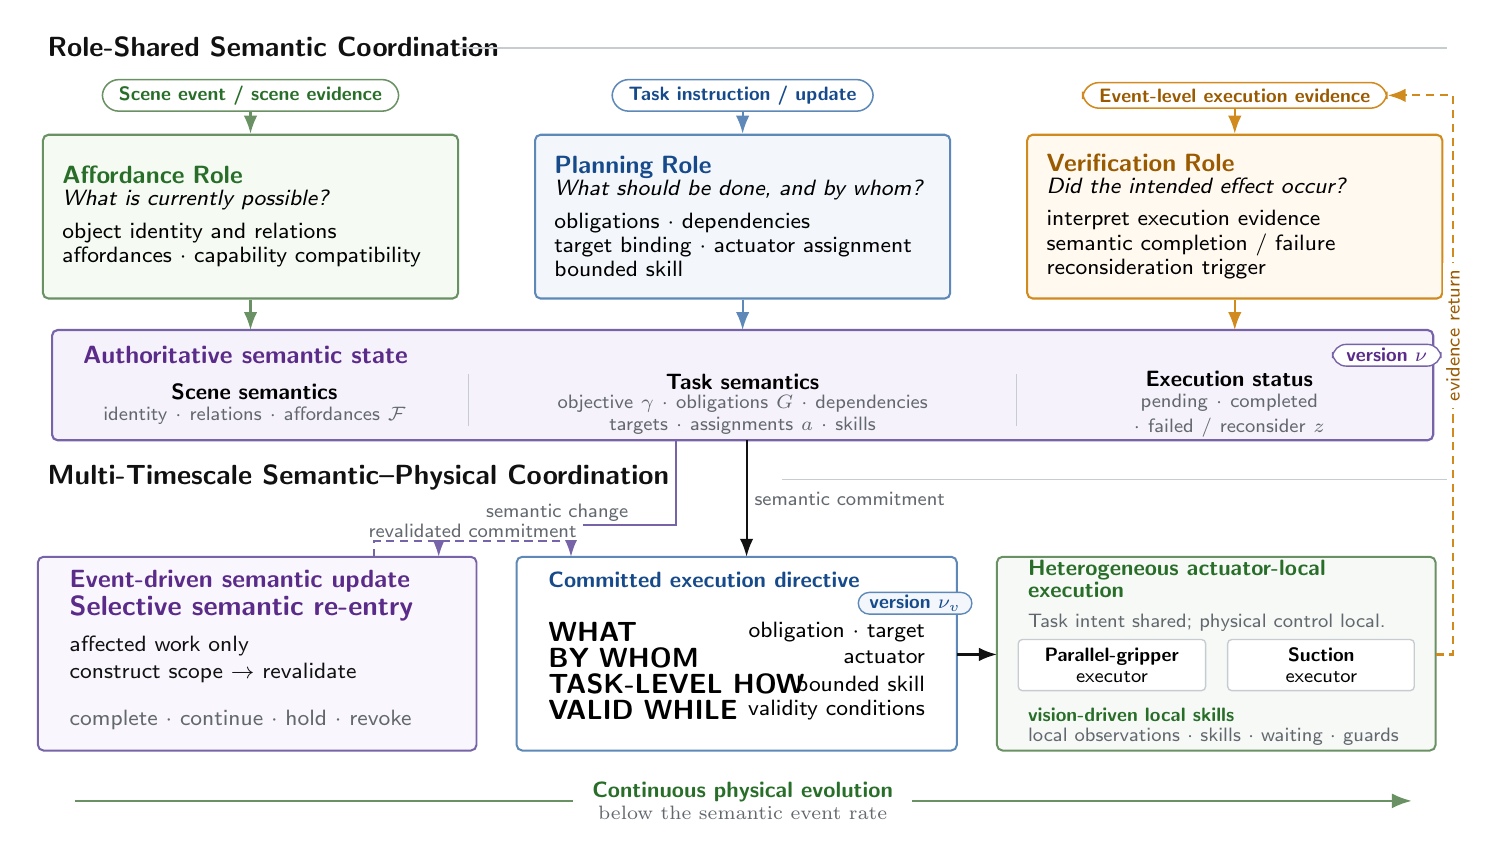
\begin{tikzpicture}[
  x=1cm,y=1cm,
  font=\sffamily\fontsize{7.8}{8.8}\selectfont,
  >=Latex,
  role/.style={draw,rounded corners=2pt,line width=0.75pt,align=left,
               inner xsep=7pt,inner ysep=6pt,text width=4.78cm,
               minimum height=2.08cm},
  input/.style={draw,rounded corners=6pt,line width=0.55pt,fill=white,
                align=center,inner xsep=6pt,inner ysep=2.2pt,
                font=\sffamily\bfseries\fontsize{7.2}{8}\selectfont},
  lower/.style={draw,rounded corners=2pt,line width=0.72pt,align=left,
                inner xsep=7pt,inner ysep=6pt,minimum height=2.28cm},
  flow/.style={-Latex,line width=0.78pt,draw=ink},
  evidence/.style={-Latex,dash pattern=on 3pt off 2pt,
                   line width=0.78pt,draw=verifyline},
  reentry/.style={-Latex,dash pattern=on 3pt off 2pt,
                  line width=0.78pt,draw=stateline},
  connectorlabel/.style={fill=white,inner xsep=2.5pt,inner ysep=1pt,
                         font=\sffamily\fontsize{6.9}{7.6}\selectfont,
                         text=muted,align=center},
  sectiontitle/.style={anchor=west,font=\sffamily\bfseries
                       \fontsize{10.2}{11}\selectfont,text=ink}
]
  % Fold I: role-owned semantic coordination.
  \node[sectiontitle] at (0.25,10.10) {Role-Shared Semantic Coordination};
  \draw[hairline,line width=0.55pt] (5.58,10.08) -- (18.15,10.08);

  \node[input,draw=affline,text=afftext] (sceneevent) at (2.95,9.48)
    {Scene event / scene evidence};
  \node[input,draw=planline,text=plantext] (taskevent) at (9.20,9.48)
    {Task instruction / update};
  \node[input,draw=verifyline,text=verifytext] (evidenceevent) at (15.45,9.48)
    {Event-level execution evidence};

  \node[role,fill=afffill,draw=affline] (affordance) at (2.95,7.94)
    {{\color{afftext}\bfseries\fontsize{9.5}{10.2}\selectfont Affordance Role}\\[-1pt]
     \textit{What is currently possible?}\\[3pt]
     object identity and relations\\
     affordances $\cdot$ capability compatibility};

  \node[role,fill=planfill,draw=planline] (planning) at (9.20,7.94)
    {{\color{plantext}\bfseries\fontsize{9.5}{10.2}\selectfont Planning Role}\\[-1pt]
     \textit{What should be done, and by whom?}\\[3pt]
     obligations $\cdot$ dependencies\\
     target binding $\cdot$ actuator assignment\\
     bounded skill};

  \node[role,fill=verifyfill,draw=verifyline] (verification) at (15.45,7.94)
    {{\color{verifytext}\bfseries\fontsize{9.5}{10.2}\selectfont Verification Role}\\[-1pt]
     \textit{Did the intended effect occur?}\\[3pt]
     interpret execution evidence\\
     semantic completion / failure\\
     reconsideration trigger};

  \draw[flow,draw=affline] (sceneevent) -- (affordance);
  \draw[flow,draw=planline] (taskevent) -- (planning);
  \draw[flow,draw=verifyline] (evidenceevent) -- (verification);

  % One authoritative state, visually shared by all three roles.
  \path[draw=stateline,fill=statefill,rounded corners=2pt,line width=0.78pt]
    (0.43,5.10) rectangle (17.97,6.50);
  \node[anchor=west,text=statetext,font=\sffamily\bfseries
        \fontsize{9.2}{10}\selectfont] at (0.70,6.18)
    {Authoritative semantic state};
  \node[draw=stateline,fill=white,rounded corners=5pt,line width=0.5pt,
        inner xsep=5pt,inner ysep=1.5pt,text=statetext,
        font=\sffamily\bfseries\fontsize{7}{7.7}\selectfont]
        at (17.38,6.18) {version $\nu$};

  \node[align=center,text width=4.7cm] at (3.00,5.56)
    {\textbf{Scene semantics}\\[-1pt]
     {\color{muted}\fontsize{7.1}{7.8}\selectfont
      identity $\cdot$ relations $\cdot$ affordances $\mathcal{F}$}};
  \node[align=center,text width=6.5cm] at (9.20,5.56)
    {\textbf{Task semantics}\\[-1pt]
     {\color{muted}\fontsize{7.1}{7.8}\selectfont
      objective $\gamma$ $\cdot$ obligations $G$ $\cdot$ dependencies\\[-1pt]
      targets $\cdot$ assignments $a$ $\cdot$ skills}};
  \node[align=center,text width=4.7cm] at (15.38,5.56)
    {\textbf{Execution status}\\[-1pt]
     {\color{muted}\fontsize{7.1}{7.8}\selectfont
      pending $\cdot$ completed $\cdot$ failed / reconsider $z$}};
  \draw[hairline,line width=0.5pt] (5.72,5.28) -- (5.72,5.94);
  \draw[hairline,line width=0.5pt] (12.68,5.28) -- (12.68,5.94);

  \draw[flow,draw=affline] (affordance.south) -- (affordance.south |- 6.50,6.50);
  \draw[flow,draw=planline] (planning.south) -- (planning.south |- 6.50,6.50);
  \draw[flow,draw=verifyline] (verification.south) -- (verification.south |- 6.50,6.50);

  % Fold II: event-rate semantics above continuous actuator-local execution.
  \node[sectiontitle] at (0.25,4.62)
    {Multi-Timescale Semantic--Physical Coordination};
  \draw[hairline,line width=0.55pt] (9.70,4.60) -- (18.15,4.60);

  \path[draw=stateline,fill=statefill!62,rounded corners=2pt,line width=0.72pt]
    (0.25,1.16) rectangle (5.82,3.62);
  \coordinate (semanticupdate) at (3.04,2.39);
  \node[anchor=west,text=statetext,font=\sffamily\bfseries
        \fontsize{9.0}{9.8}\selectfont] at (0.53,3.31)
    {Event-driven semantic update};
  \node[anchor=west,text=statetext,font=\sffamily\bfseries]
    at (0.53,2.96) {Selective semantic re-entry};
  \node[anchor=west,text=ink] at (0.53,2.49) {affected work only};
  \node[anchor=west,text=ink] at (0.53,2.15)
    {construct scope $\rightarrow$ revalidate};
  \node[anchor=west,text=muted] at (0.53,1.55)
    {complete $\cdot$ continue $\cdot$ hold $\cdot$ revoke};

  \path[draw=planline,fill=white,rounded corners=2pt,line width=0.72pt]
    (6.33,1.16) rectangle (11.92,3.62);
  \coordinate (directive) at (9.13,2.39);
  \node[anchor=west,text=plantext,font=\sffamily\bfseries
        \fontsize{8.3}{9.1}\selectfont] at (6.61,3.33)
    {Committed execution directive};
  \node[draw=planline,fill=planfill,rounded corners=4pt,line width=0.5pt,
        inner xsep=4pt,inner ysep=1pt,text=plantext,
        font=\sffamily\bfseries\fontsize{6.6}{7}\selectfont]
    at (11.39,3.03) {version $\nu_v$};
  \node[anchor=west,font=\sffamily\bfseries] at (6.61,2.67) {WHAT};
  \node[anchor=east] at (11.64,2.67) {obligation $\cdot$ target};
  \node[anchor=west,font=\sffamily\bfseries] at (6.61,2.34) {BY WHOM};
  \node[anchor=east] at (11.64,2.34) {actuator};
  \node[anchor=west,font=\sffamily\bfseries] at (6.61,2.01) {TASK-LEVEL HOW};
  \node[anchor=east] at (11.64,2.01) {bounded skill};
  \node[anchor=west,font=\sffamily\bfseries] at (6.61,1.68) {VALID WHILE};
  \node[anchor=east] at (11.64,1.68) {validity conditions};

  \path[draw=execline,fill=execfill,rounded corners=2pt,line width=0.72pt]
    (12.43,1.16) rectangle (18.00,3.62);
  \coordinate (execution) at (15.22,2.39);
  \node[anchor=west,text=afftext,align=left,
        font=\sffamily\bfseries\fontsize{8.5}{9.2}\selectfont]
    at (12.70,3.34) {Heterogeneous actuator-local\\[-1pt]execution};
  \node[anchor=west,text=muted,font=\sffamily\fontsize{7.1}{7.8}\selectfont]
    at (12.70,2.79) {Task intent shared; physical control local.};
  \path[draw=hairline,fill=white,rounded corners=1.5pt,line width=0.5pt]
    (12.70,1.92) rectangle (15.08,2.57);
  \path[draw=hairline,fill=white,rounded corners=1.5pt,line width=0.5pt]
    (15.36,1.92) rectangle (17.73,2.57);
  \node[align=center,font=\sffamily\fontsize{7}{7.7}\selectfont]
    at (13.89,2.245) {\textbf{Parallel-gripper}\\executor};
  \node[align=center,font=\sffamily\fontsize{7}{7.7}\selectfont]
    at (16.55,2.245) {\textbf{Suction}\\executor};
  \node[anchor=west,text=afftext,font=\sffamily\bfseries
        \fontsize{7.2}{7.9}\selectfont] at (12.70,1.62)
    {vision-driven local skills};
  \node[anchor=west,text=muted,font=\sffamily\fontsize{6.8}{7.4}\selectfont]
    at (12.70,1.34) {local observations $\cdot$ skills $\cdot$ waiting $\cdot$ guards};

  \draw[flow,draw=stateline]
    (8.35,5.10) -- (8.35,4.02) --
    node[connectorlabel,above]{semantic change}
    (5.34,4.02) -- (5.34,3.62);
  \draw[flow]
    (9.25,5.10) -- node[connectorlabel,right]{semantic commitment}
    (9.25,3.62);
  \draw[reentry]
    (4.52,3.62) -- (4.52,3.82) --
    node[connectorlabel,above]{revalidated commitment}
    (7.02,3.82) -- (7.02,3.62);
  \draw[flow]
    (11.92,2.38) -- (12.43,2.38);

  % Event-level evidence is the only upward return from physical execution.
  \draw[evidence]
    (18.00,2.38) -- (18.22,2.38) -- (18.22,9.48) --
    (evidenceevent.east);
  \node[connectorlabel,text=verifytext,rotate=90] at (18.22,6.43)
    {evidence return};

  \draw[-Latex,line width=0.95pt,draw=execline]
    (0.72,0.52) -- (17.70,0.52);
  \node[fill=white,inner xsep=7pt,inner ysep=1.5pt,align=center,
        text=afftext,font=\sffamily\bfseries\fontsize{8.2}{9}\selectfont]
    at (9.20,0.52)
    {Continuous physical evolution\\[-1pt]
     {\normalfont\color{muted}\fontsize{6.9}{7.5}\selectfont
      below the semantic event rate}};

  % Stable bounding box for predictable manuscript scaling.
  \path[use as bounding box] (0.12,0.15) rectangle (18.38,10.34);
\end{tikzpicture}
\end{document}
